
\begin{enumerate}


\item If the sum of zeroes of the polynomial $ p\brak x = 2x^2 - k\sqrt2x+1 $ is${\sqrt2} $,then value of k is:
\begin{enumerate}
    \item $ \sqrt{2} $
    \item $2$
    \item $ 2  \sqrt{2} $
    \item $ \frac{1}{2} $
 \end{enumerate}

\item If the roots of the equation $ax^2 + bx + c = 0$,$a \neq 0$ are real and equal, then which of the following relations is true?
\begin{enumerate}    
    \item $a = \frac{b^2}{c}$
    \item $b^2 = ac$                                                                                    \item $ac = \frac{b^2}{4}$
    \item $c = \frac{b^2}{a}$
\end{enumerate}

\item In an A.P., if the first term $a = 7$, $n$th term $a_{n} = 84$, and the sum of the first $n$ terms $s_{n} = \frac{2093}{2}$, then $n$ is equal to:
\begin{enumerate}
    \item $22$
    \item $24$
    \item $23$
    \item $26$
\end{enumerate}

\item The zeroes of a polynomial $x^2 + px + q$ are twice the zeroes of the polynomial $4x^2 - 5x - 6$. The value of $p$ is:
	\begin{enumerate}   
\item $-\frac{5}{2}$
    \item $\frac{5}{2}$
    \item $-5$
    \item $10$
	\end{enumerate}
\newpage
 \item In the given figure, graphs of two linear equations are shown. The pair of these linear equations is:
\begin{figure}[!ht]
\centering
\includegraphics[width=\columnwidth]{figs/Image1.jpg}
\caption{}
\label{fig:enter-label}
\end{figure}
\begin{enumerate}
    \item consistent with a unique solution.
    \item consistent with infinitely many solutions.
    \item inconsistent.
    \item inconsistent but can be made consistent.
\end{enumerate}

\item solve the following system of linear equcations $7x-2y=5$ and verify your answer.
\item A rectangular floor area can be completely tiled with $200square$ tiles. If the side length of each tile is increased by $1$ unit, it would take only $128$ tiles to cover the floor.
\begin{figure}[!ht]
\centering
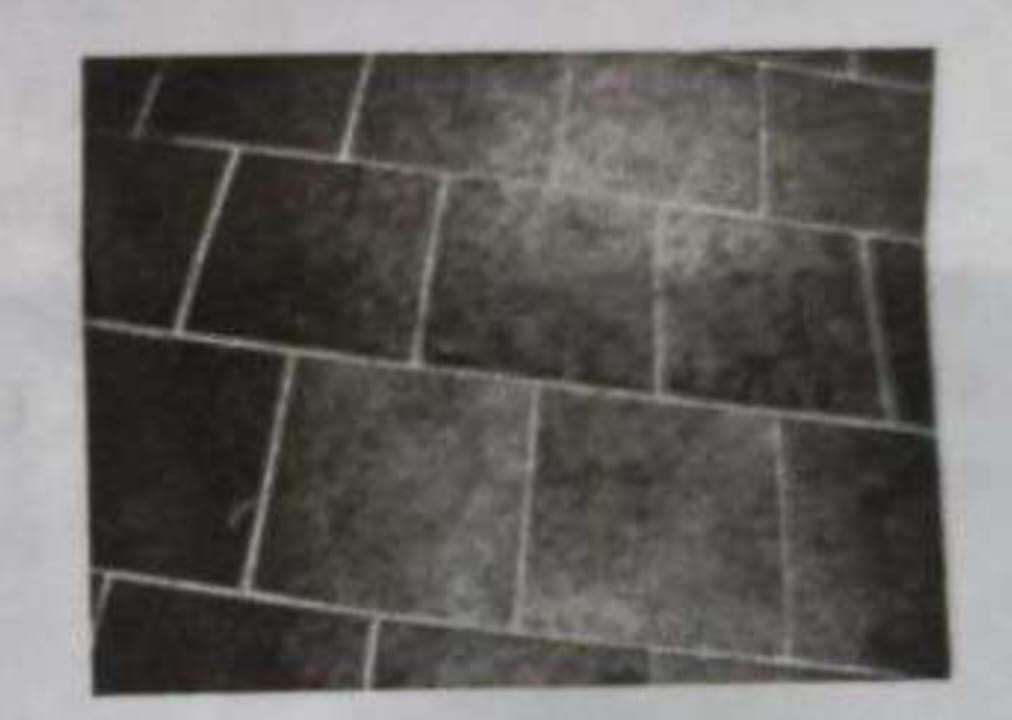
\includegraphics[width=\columnwidth]{figs/a1.jpg}
\label{fig:image5}
\caption{image5}
\end{figure}
\begin{enumerate}
\item Assuming the original length of each side of a tile be x units, make a quadratic equation from the above information.\
\item Write the corresponding quadratic equation in standard form.\
\item Find the value of x, the length of side of a tile by factorisation.
\end{enumerate}
\item solve the quadratic equcation for x, using quardratic formula.
\item \textbf{Assertion (A):} If the graph of a polynomial touches x-axisat only one point, then the polynomial cannot be a quadratic polynomial.

\textbf{Reason (R):} A polynomial of degree $n\brak{n > 1}$ can have at most n zeroes.
\item  The sum of first and eights of an A.P. is $32$ and their product is $60$. Find the first term  and co
mmon difference of the A.P. Hence,also find the sum of its first $20$ terms.
\item In an A.P. of $40$ terms, the sum of first $9$ terms is $153$ and the sum of last $6$ terms is $687$.
Determine the first term and common difference of A.P. Also, find the sum of all the terms of the A.P.





\end{enumerate}
